%*******************************************************************************
% Copyright (c) 2014 Formal Mind GmbH and others
% All rights reserved. This program and the accompanying materials
% are made available under the terms of the Eclipse Public License v1.0
% which accompanies this distribution, and is available at
% http://www.eclipse.org/legal/epl-v10.html
% 
% Contributors:
%     Michael Jastram - initial Copy
%     Maha Jastram - susequent improvements
%******************************************************************************/

% ===================================================================================
\section{Basic Concepts}
\label{sec:tutorial-basic-concepts}
\index{concepts}
% ===================================================================================

In this tutorial, we will use the ReqIF terminology, which can be confusing.  Therefore, please familiarize yourself with the terminology first (Section~\ref{sec:terminology}).

\begin{warning}
In ReqIF terminology, a requirement is called \term{SpecObject}, a link is a \term{SpecRelation}, and the document view consists of \term{SpecHierarchies}.  Confused? Then please have a look at Section~\ref{sec:terminology}, where the terminology is described.
\end{warning}

% ===================================================================================
\section{Tutorial 1: Creating a Basic ReqIF Model}
\label{sec:tutorial-create-basic-model}
% ===================================================================================

In this section, we will build a ReqIF model from scratch, step by step.

% -----------------------------------------------------------------------------------
\subsection{Install \pror{}}
\label{sec:install-reqif-studio}
\index{installation}
% -----------------------------------------------------------------------------------

The easiest way for installing \pror{} is downloading \href{https://reqif.academy}{ReqIF Studio}.  This is a standalone-application that is based on Eclipse RMF, combined with some enhancements.

 Alternatively, you can install RMF in any Eclipse-Installation via its update site (listed on the \href{https://www.eclipse.org/rmf/download.php}{RMF Download page}).  This is recommended for advanced users only who need to integrate RMF with other Eclipse-based components.

\begin{info}
The installation is described in detail in Section~\ref{sec:installation}.
\end{info}

% -----------------------------------------------------------------------------------
\subsection{Create the Model}
\label{sec:create-model}
\index{create ReqIF model}
\index{ReqIF model!create}
% -----------------------------------------------------------------------------------

\begin{itemize}

\item
  If you do not already have one, create a new \term{project}: Select  \menu{File | New | Project};
\item
  Create the ReqIF model by selecting \menu{File | New | Reqif10 Model};
\item
  Select the project and name the file ``tutorial.reqif''.  Click \menu{Finish};
\item
  Upon completion, the model will be opened, as well as the one and only \menu{Specification} contained in this model.
\end{itemize}

After this, your window should look more or less as shown in Figure~\ref{fig:pror_gui}.

\begin{figure}
  \centering
  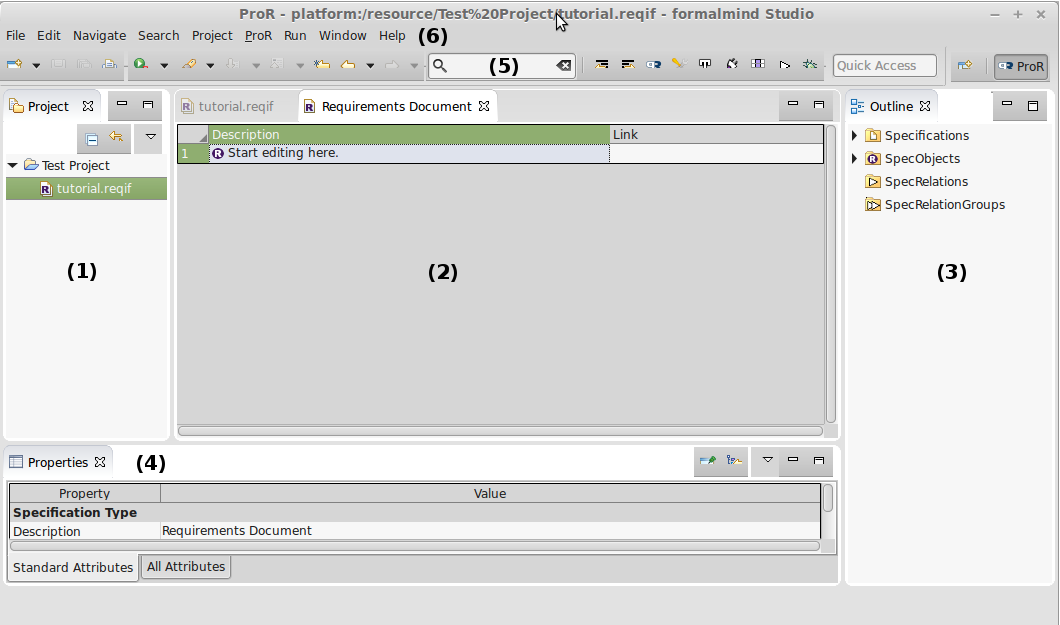
\includegraphics[width=\linewidth]{../rmf-images/Screenshot_intro.png}
  \caption{The \pror{} user interface}
  \label{fig:pror_gui}
\end{figure}

You will see your ReqIF file in the \menu{Project Explorer} window (1).

The \menu{Specification Editor} (2) shows your \term{Specifications}.

In the Specification Editor, you see the \term{SpecObjects} that exist in this Specification.  There is currently only one, with the description ``Start editing here''.

The \menu{Outline} (3) has four folders:
\index{outline view}

\begin{description}
\item[Specifications.] Shows the Specifications in the ReqIF.  You can expand the tree to expose the hierarchy of SpecObjects in the ReqIF model.
\item[SpecObjects.] Shows all SpecObjects in the ReqIF model as a flat list.  Keep in mind that SpecObjects in Specifications are references.  In contrast, this folder shows all SpecObjects created for the ReqIF model, whether or not they are referenced.
\item[SpecRelations.] Shows all SpecRelations in the ReqIF as a flat list.  For now, we will ignore SpecRelations.
\item[SpecRelationsGroups.] These are special constructs that can be used for grouping SpecRelations with the same source and target.
\end{description}

The properties of a selected \term{SpecElement} are shown in the \menu{Properties View} (4).  As the only SpecObject in the model is selected, we see its \term{SpecType} (``Requirements Type'') and its only \term{Attribute} (``Description'') with the value ``Start editing here.''  There are two tabs \menu{Standard Attributes} and \menu{All Attributes} at the bottom of the \menu{Properties View}.  The \menu{Standard Attributes} tab shows you all standard attributes of the selected element.  \menu{All Attributes} shows all existing ReqIF attributes of the selected element.

Above the main working windows it the tool bar (5) and, at the very top, the menu bar (6).

% -----------------------------------------------------------------------------------
\subsection{Customizing the SpecType}
\label{sec:customize-spec-type}
\index{SpecType configuration}
\index{datatype configuration}
\index{configuration!SpecType}
\index{configuration!datatype}
% -----------------------------------------------------------------------------------

To get familiar with the tool, we will:

\begin{itemize}
\item
  Add two more attributes to the SpecObjectType called ``ID'' and ``Owner'' and
\item
  We will show those \term{Attributes} in the \term{Specification}
\end{itemize}

The results of this are shown in Figure~\ref{fig:datatype_configuration}.

\begin{figure}
\centering
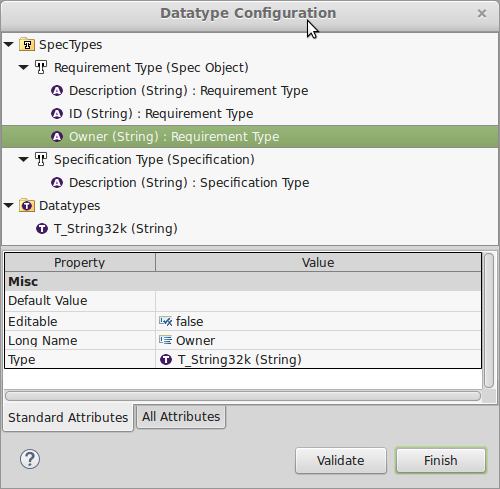
\includegraphics[width=0.8\linewidth]{../rmf-images/datatype.png}
\caption{Datatype Configuration Dialog}
\label{fig:datatype_configuration}
\end{figure}

To add new attributes, we open the \menu{Datatype Configuration} dialog with \menu{Studio | Datatype Configuration}.  Alternatively you can also click on 
\includegraphics[height=0.8em]{../rmf-images/icons/full/obj16/SpecType.png} in the Tool Bar.

The resulting dialog box has two folders in the upper pane: one for \term{SpecTypes} and one for \term{Datatypes}.  Currently, there is only one Datatype ``T\_String32k'' and two SpecTypes, one called ``Requirements Type'' with the attribute ``Description'' and one called ``Specification Type'' with the attribute ``Description''.

In the lower pane are the details in regards to each attribute.

We add more Attributes to ``Requirements Type'' by right-clicking it and selecting \menu{New Child | Attribute Definition String}.  This will create a new element.  Upon selecting it, we can rename it and tailor the details.  Double-click on the ``Long Name'' variable and type in ``ID''.  Change the Type by double-clicking the field and choosing ``T\_String32k'' from the dropdown menu.  Repeat the process but this time change the ``Long Name'' to ``Owner''.  In the end, the dialog should look as shown in Figure~\ref{fig:datatype_configuration}.

Upon closing the dialog, little will have changed - the Specification still shows just two columns, Description and Link.  However, if you select the requirement, you will see the new Properties (ID and Owner) in the Property view.

% -----------------------------------------------------------------------------------
\subsection{Showing the New Attributes}
\label{sec:show-new-attributes}
\index{configuration!columns}
\index{column configuration}
% -----------------------------------------------------------------------------------

\begin{figure}
\centering      
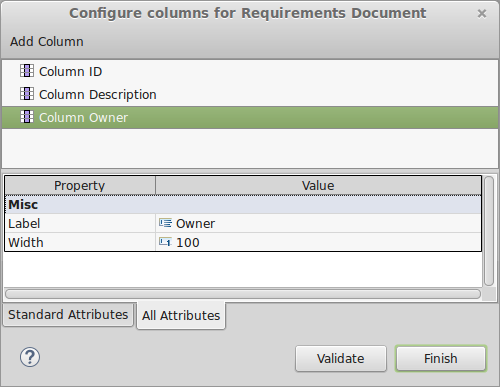
\includegraphics[width=0.8\linewidth]{../rmf-images/columnconfig.png}      
\caption{Column Configuration}
\label{fig:column_configuration}
\end{figure}

To show the new Attributes in the Specification, we have to configure the columns shown in the \menu{Specification Editor}.  We do this by selecting \menu{Studio | Column Configuration}.  You can also click on 
\includegraphics[height=0.8em]{../rmf-images/icons/full/obj16/Column.png} in the Tool Bar.

The resulting Dialog shows one entry, ``Description'' for the one and only Column of the Specification.  In the ``Value'' column double click on ``Description to choose it and replace it with ``ID''.

By clicking on the ``Add Column'' icon at the top of the dialog, create a new column and name it ``Description''.  In this view, the columns can be dragged and dropped to change their order as desired.

The resulting window is shown in Figure~\ref{fig:column_configuration}.

\begin{info}
Note that you have to provide free text for the columns for the same reason that we used free text for the ``Labels'' earlier: This way we can easily match multiple SpecObjects of different types.
\end{info}

You can actually adjust the width of the columns simply by dragging the column headers.

% -----------------------------------------------------------------------------------
\subsection{Adding new SpecObjects}
\label{sec:add-specobjects}
\index{SpecObjects!create}
\index{create!SpecObjects}
% -----------------------------------------------------------------------------------

\begin{figure}
\centering
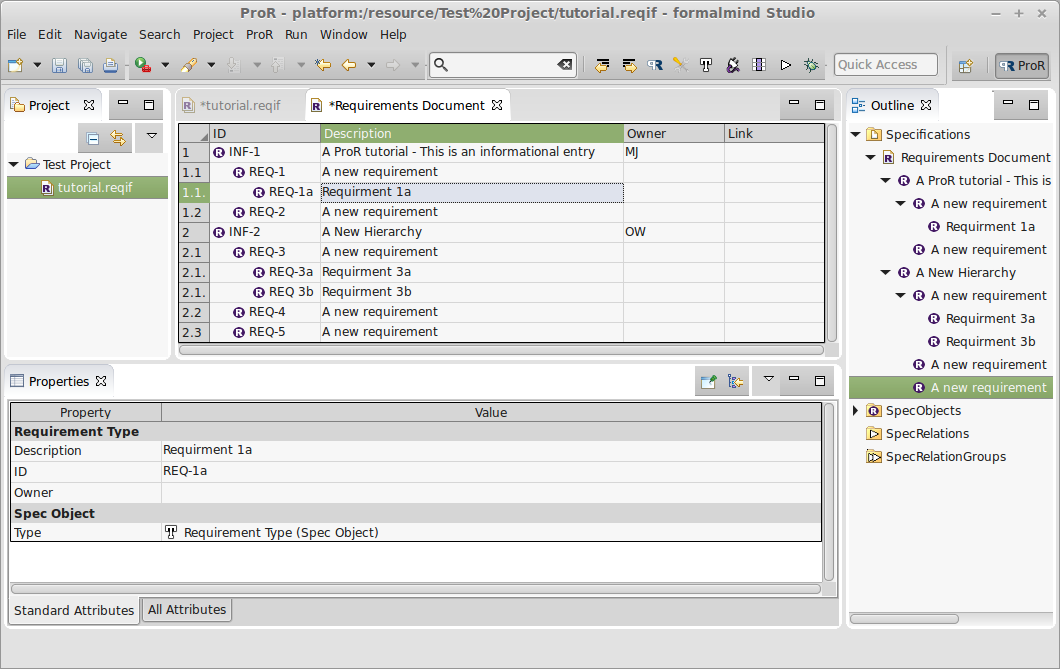
\includegraphics[width=\linewidth]{../rmf-images/hierarchy_example.png}      
\caption{Adding SpecObjects}      
\label{fig:requirements_hierarchy}
\end{figure}

Now we can finally add \term{SpecObjects} by right-clicking on a row in the Specification View.  In the context-menu, there are two submenus: \menu{New Child} and \menu{New Sibling}.

In both menus, there are three entries \menu{Spec Hierarchy}, \menu{SpecObject} and \menu{SpecObject (Requirement Type)}.  Some background is needed here:

\index{SpecHierarchy}
We said before that Specifications contain references to SpecObjects.  A \menu{SpecHierarchy} is the wrapper that allows the hierarchical structure and that points to the referenced SpecObject.  Usually, we don't have to be concerned with them.  Therefore the second option: If selected, a new SpecHierarchy is created and associated with a new SpecObject, which in turn is set immediately to the given \term{SpecType}.  If we had more than just one SpecType (besides ``Requirements Type''), there would be an entry for each SpecType in the context menu.

To continue the exercise, select the \menu{New Child | SpecObject (Requirement Type)}.  Now we have two SpecObjects.  The original is numbered on the far left-hand side of the pane with a ``1''.  The second one, the child, is numbered ``1.1''.  Now we should change the ID's of each entry.  Click in the cell of the column ``ID`` (in row 1) and type in INF-1.  Under Description, type ''A ReqIF tutorial.``  For the second, change the ID to REQ-1 and ''Learn how to create a new requirement'' in the ``Description'' column.

Feel free to add a few more rows and or even new structures.  Yours should look somethinig similar to Figure~\ref{fig:requirements_hierarchy}.

% -----------------------------------------------------------------------------------
\subsection{Rearranging Elements}
\label{sec:rearrange-elements}
\index{SpecObjects!rearrange}
% -----------------------------------------------------------------------------------

\begin{figure}
\centering
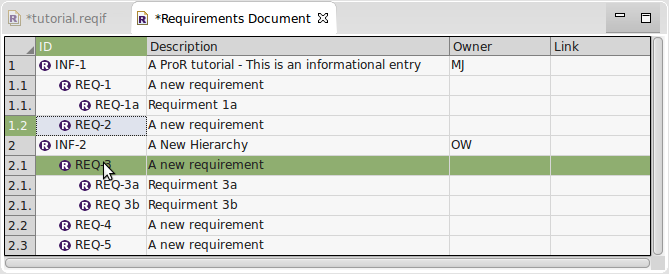
\includegraphics[width=0.8\linewidth]{../rmf-images/draganddrop.png}    
\caption{Drag and Drop}      
\label{fig:dragAndDropChild}
\end{figure}

SpecObjects can be reordered by using drag and drop.  This works both in the \menu{Specification View} and the \menu{Outline View}.

You can drag and drop a SpecObject as a sibling or a child.  The highlighting feedback will enable you to see what you're moving and where to.  For instance, if you are dragging a SpecObject over another one, the entire cell will be highlighted.  This means, that the SpecObject will be assigned as a child to the dropped SpecObject.

If you are dragging a SpecObject between two rows, you also get visual feedback on whether the SpecObject will be assigned as a sibling.

Figure~\ref{fig:dragAndDropChild} shows drag and drop in action.

You can also move elements by using cut and paste.  Pasting will insert an element as a child.

% -----------------------------------------------------------------------------------
\subsection{Export Specification as HTML}
\label{sec:export-specs}
\index{printing}
\index{HTML export}
% -----------------------------------------------------------------------------------

If you want to export your Specification as HTML, open the Specification you would like to export and initiate printing \menu{File | Print...}.  The HTML representation is generated and opened in your system's web browser.

% -----------------------------------------------------------------------------------
\subsection{Conclusion}
\label{sec:tutorial-conclusion}
% -----------------------------------------------------------------------------------

Quite an achievement—but there's still a bit of a way to go.  One improvement we can make is simplifying data entry.  Another is improving  the visibility of the descriptions.  In the next part of the tutorial, we will address these issues.

% ===================================================================================
\section{Tutorial 2: Use Presentations}
\label{sec:tutorial-presentations}
\index{presentation}
\index{plugin}
% ===================================================================================

We will continue where we left off at the end of Tutorial 1 and we will assume that you have \pror{} open with a model identical or similar to the one we created earlier.

In this tutorial we will introduce \term{Presentations}.  Presentations are Eclipse Plug-Ins that extend the functionality of \pror{}.  Specifically:

\begin{itemize}
\item
  Presentations can change the way Attributes are rendered in the Specification,
\item
  Presentations can change the way Attributes are edited in the Specification and
\item
  Presentations can perform tasks in the background.
\end{itemize}

\pror{} comes with a number of standard presentations that we will introduce in this tutorial.

\begin{figure}
\centering      
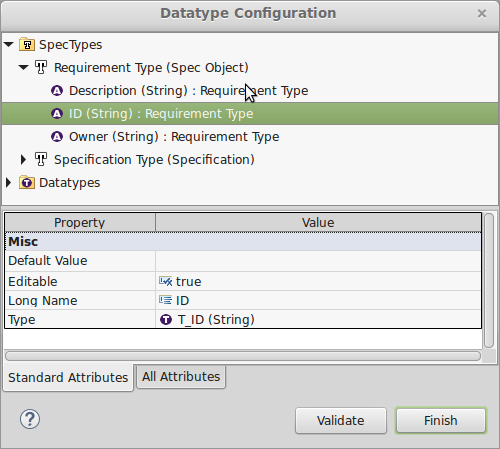
\includegraphics[width=0.8\linewidth]{../rmf-images/t_id.png}      
\caption{Datatype Configuration Dialog}      
\label{fig:datatypeConfig}
\end{figure}

% -----------------------------------------------------------------------------------
\subsection{ID Presentation}
\label{sec:id-presentation}
\index{create!IDs}
\index{ID creation}
% -----------------------------------------------------------------------------------

It would be nice if every SpecObject had its own unique ID.  Actually, they do: The unique ID is shown in the \menu{All Attributes} tab of the \menu{Property View}, if a SpecObject is selected.  But that ID is meant for machines and is not practical.

The ID Presentation allows the automatic creation of more user-friendly IDs.  Let's create one.

Remember that Presentations are associated with \term{Datatypes}, not \term{Attributes}.  Thus, we first have to create a new Datatype called ``T\_ID``.  We then associate that Datatype with the Attribute ``ID''.  We described this process in the first tutorial.  Figure~\ref{fig:datatypeConfig} shows the configuration dialog, when all is done.

The next step is the association of the Datatype with the Presentation.

\begin{figure}
\centering      
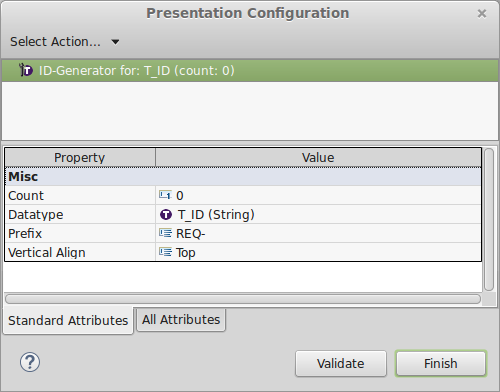
\includegraphics[width=0.8\linewidth]{../rmf-images/presentation_id.png}      
\caption{Configuration of the ID Presentation}
\label{fig:idConfig}
\end{figure}

We open the Presentation Configuration and create a new Presentation from the dropdown menu \menu{Select Action...}, of type ``Id'' Presentation.  We associate it with the newly created Datatype.  After configuration, it would look as shown in Figure~\ref{fig:idConfig}.

Note that you can adjust the prefix, count and the vertical alignment of the presentation.

\begin{warning}
At this point, the Presentation does not yet check for duplicates.  It simply grabs a new value from count, increments it and uses it.  Also, existing values are never overwritten.
\end{warning}

% ===================================================================================
\section{Tutorial 3: Advanced SpecTypes}
\label{sec:tutorial-spec-types}
% ===================================================================================

So far, we have a model with only one SpecObjectType.  In this tutorial, we will show how we can work with multiple SpecTypes, and we will introduce other SpecTypes.

% -----------------------------------------------------------------------------------
\subsection{Multiple SpecTypes}
\label{sec:multiple-spec-types}
% -----------------------------------------------------------------------------------

The first entry in our Specification (``A ReqIF Tutorial'') isn't really a requirement.  Thus, it doesn't need an ID or an owner, and it would be nice to highlight it somehow.  For highlighting, we have the \menu{Headline Presentation}.  We will:

\begin{itemize}

\item
  Create a new \term{SpecType} for headlines.
\item
  Create a new \term{Datatype} that will be used for the headline content.
\item
  Associate that Datatype with the \menu{Headline Presentation}.
\end{itemize}

\begin{figure}
\centering      
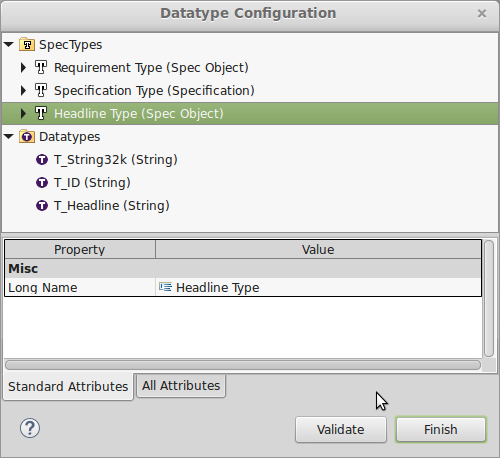
\includegraphics[width=0.8\linewidth]{../rmf-images/datatype_Headline_desc.png}      
\caption{Datatype Configuration for the Headline Presentation}      
\label{fig:headlineConfig}
\end{figure}

By selecting \menu{Studio | Datatype Configuration}, we open the dialog where we can create new SpecTypes and Datatypes.  For the first time, we create a new SpecType by right-clicking on \menu{SpecTypes}.  One of the entries in the child menu is \menu{SpecObject Type}.

Once created, we select it and rename as ``Headline Type'' in the \menu{Property Pane}.

Then we give it a new Attribute called ``Description'' by right-clicking it and selecting \menu{String}.

\begin{warning}
It is important that we call it ``Description''.  This matches the Attribute name from ``Requirement Type''.  By using the same name, we ensure that the Attributes \textbf{appear in the same column}, even though they are different Attributes from different SpecTypes.
\end{warning}

We do not set the type yet, as we need to create a new Datatype.  We do this, as before, by right-clicking on the \menu{Data\-types} folder in the upper pane.  Create a child of type \menu{Definition String}.  Call it ``T\_Headline'' and set the length to 50.  Now we can go back to the ``Description'' Attribute (in the upper pane) and set the type to T\_Headline, which is now available from the dropdown.

When all this is done, the resulting configuration should look as shown in Figure~\ref{fig:headlineConfig}.

You can change the type of a SpecObject by selecting it and changing it in the \menu{Properties View}.  Please note that currently all existing values are lost when changing the type.

Note the following:

\begin{figure}
\centering      
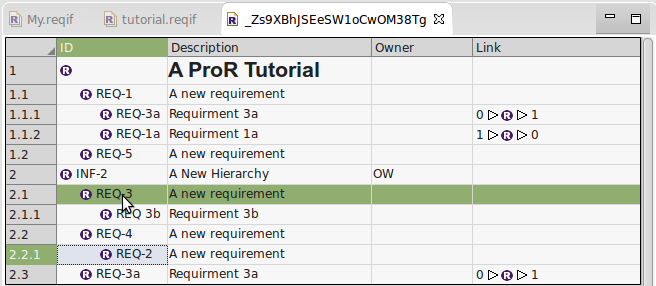
\includegraphics[width=0.8\linewidth]{../rmf-images/hierarchy_step_1}
\caption{Activated Headline Configuration}      
\label{fig:activeHeadlineConfig}
\end{figure}

\begin{itemize}
\item
  For SpecObjects of this SpecType, the columns ``ID'' and ``Owner'' are now empty and cannot be edited.
\item
  Note how the \menu{Property View} changes as you select SpecObjects of different SpecTypes.
\item
  Right-clicking on a row now shows one more option for child/sibling creation: A new entry of type ``Headline Type''.
\item At this point, the description of the headline is not yet formatted, as we have not activated the Presentation yet.
\end{itemize}

\begin{figure}
\centering      
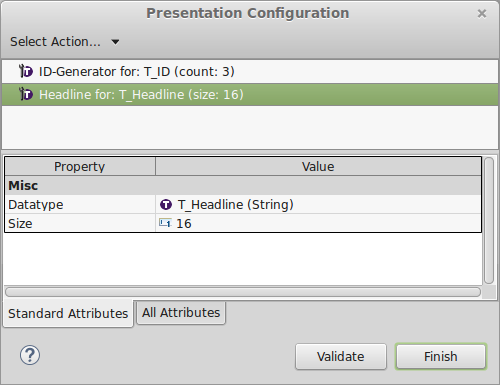
\includegraphics[width=0.8\linewidth]{../rmf-images/Presentation_headline.png}      
\caption{Presentation Configuration for Headline}      
\label{fig:headlineConfig2}
\end{figure}

Last, we will create a \menu{Headline Presentation} and activate it for the type ``T\_Headline''.  This is done via the \menu{Presentation Configuration}, as before.  The configuration allows you to change the font size of the headline in the ``Size'' property.  The presentation configuration is shown in Figure~\ref{fig:headlineConfig2}.

After all the changes, the Specification should look as shown in Figure~\ref{fig:activeHeadlineConfig}.  Note that the formatting is also applied in the \menu{Properties View}.

% -----------------------------------------------------------------------------------
\subsection{Other SpecTypes}
\label{sec:other-spec-types}
% -----------------------------------------------------------------------------------

\begin{figure}
\centering      
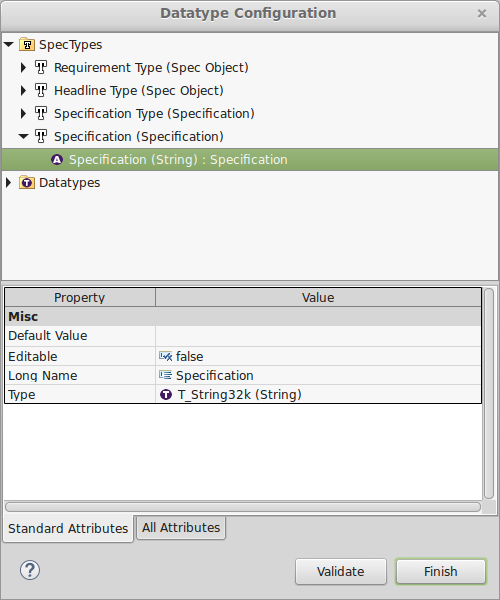
\includegraphics[width=0.8\linewidth]{../rmf-images/new_spectype.png}      
\caption{Creating a New SpecType}      
\label{fig:newSpecType}
\end{figure}

You may have noticed in the \menu{Datatype Configuration Dialog}, that right-clicking on \menu{SpecTypes} offered more options, besides \menu{SpecObject Type}.  A number of Elements can have Attributes, not just SpecObjects.

We will now create a \term{SpecificationType} and assign it to our Specification.

Try to create a SpecificationType and configure it as shown in Figure~\ref{fig:newSpecType}:

Next, we will assign this type to the one Specification that we have.  To do this we select the Specification in the \menu{Outline View} (first element in the Folder \menu{Specifications}).  That will show
the Specification's properties in the \menu{Properties View}.  The \menu{Type} property is empty.  We select ``Specification Type'' from the dropdown.

As soon as it is selected, the Attribute ``Description'' will appear in the Properties View, as now the Specification has an attribute of that name.  If we set it to a meaningful name, the label in the Outline View will change as well.

% ===================================================================================
\section{Tutorial 4: Links Between Elements}
\label{sec:tutorial-links}
\index{create!SpecRelations}
% ===================================================================================

A central feature of professional requirements tools is the ability to connect requirements with each other.  These are typically called links, traces or relations.  In ReqIF, these are \term{SpecRelations}.

% -----------------------------------------------------------------------------------
\subsection{Creating SpecRelations}
\label{sec:create-links}
% -----------------------------------------------------------------------------------

There are two ways of creating SpecRelations: (1) via the context menu and (2) via drag and drop.

\begin{info}
We recommend to use the context menu for linking.  It works even if source and target are not visible, it allows n:m linking, and it allows for the assignment of a SpecType to the newly created SpecRelations in one step.
\end{info}



% -----------------------------------------------------------------------------------
\subsection{Linking Via Context Menu}
\label{sec:context-links}
% -----------------------------------------------------------------------------------

Linking via context menu happens in two steps: initiating linking and completing linking.

Linking is initiated by right-clicking on one SpecObject, or a selection of SpecObjects.  The context menu contains the option \menu{Initiate Linking}, with a number in parentheses. The number indicates the count of affected SpecObjects.

Linking can only be completed if it has been initiated.  In that case, right-clicking on a single SpecObject or a selection of SpecObjects will show two more entries in the context menu.  These are \menu{Complete Linking To Selection} and \menu{Complete Linking From Selection}.  It will also indicate in parentheses with how many SpecObjects the linking had been initialized.

Each of these entries has a submenu, listing all SpecTypes for SpecRelations.  By selecting the appropriate option, SpecRelations will be created between the two sets of SpecObjects.  The SpecRelations will have the selected SpecType.

% -----------------------------------------------------------------------------------
\subsection{Linking Via Drag and Drop}
\label{sec:drag-links}
% -----------------------------------------------------------------------------------

SpecRelations are also be created by ``Link-Dragging''.  This is platform specific:

\begin{description}

\item
  [Linux.] Dragging with Ctrl-Shift.
\item
  [Mac.] Hold down OPTION and APPLE/COMMAND keys while dragging.
\item
  [Windows.] Dragging with Alt.
\end{description}

% -----------------------------------------------------------------------------------
\subsection{SpecRelations in the User Interface}
\label{sec:links-ui}
% -----------------------------------------------------------------------------------

\begin{figure}   
\centering      
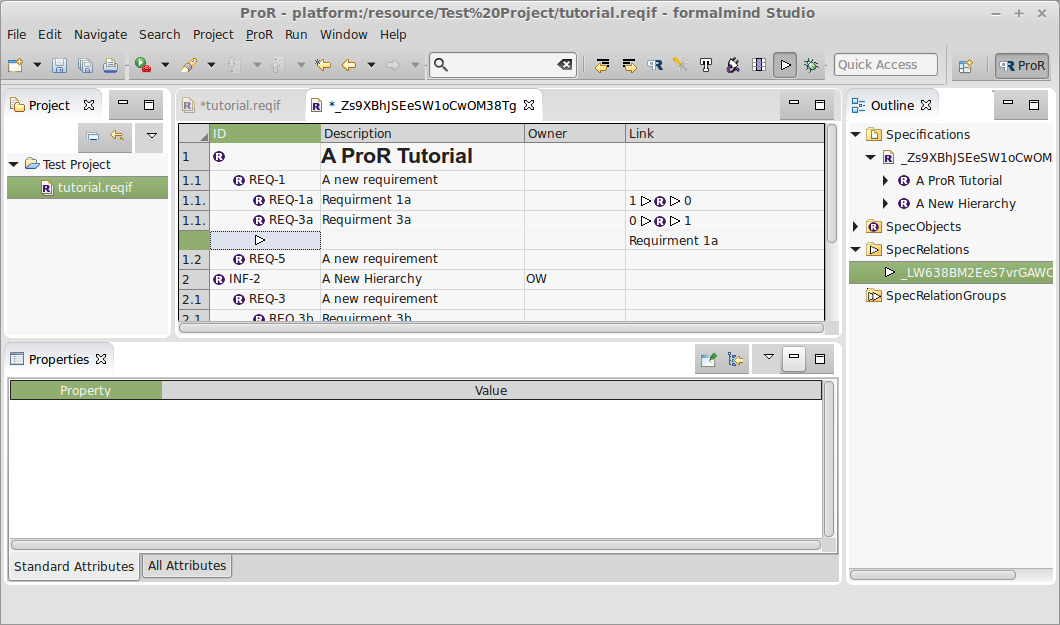
\includegraphics[width=0.8\linewidth]{../rmf-images/links.png}      
\caption{Showing Links in the GUI}      
\label{fig:linksInGui}
\end{figure}

After creating SpecRelations, the right-most column (\menu{Link}) in the \menu{Specification Editor}, has content.  It summarizes the number of incoming and outgoing SpecRelations.  The number to the left of the triangle is incoming links, the other, outgoing links (see Figure~\ref{fig:linksInGui}).

Showing SpecRelations \textbf{for a single SpecObject} can be switched on or off by double-clicking on the Link cell.

Showing SpecRelations \textbf{for all SpecObjects} can be switched on or off with the little triangle icon in the toolbar 
\includegraphics[height=0.8em]{../rmf-images/icons/full/obj16/SpecRelation.png}.

As SpecRelations can have Attributes, these are shown in the corresponding column, if the column name matches the Attribute name.  Selecting the row of a SpecRelation will show all its Attributes in the \menu{Properties View}.

The \menu{Link} cell of a SpecRelation shows the label of the link target of that SpecRelation.  Selecting it will show the link target's Attributes in the \menu{Properties View} (instead of the SpecRelation's Attributes, as for all other cells).

\begin{info}
Selecting the \menu{Link} column of a SpecRelation allows the link target to be quickly inspected.
\end{info}

Figure~\ref{fig:linksInGui} shows a Specification where REQ-1a and REQ-3a are linked.

% -----------------------------------------------------------------------------------
\subsection{Following SpecRelations}
\label{sec:follow-links}
\index{SpecRelations!follow}
\index{follow SpecRelations}
% -----------------------------------------------------------------------------------

It is possible to navigate along SpecRelations. To do so, make the links visible, as described in Section~\ref{sec:links-ui}. Double-clicking on the label of the link target will open the appropriate Specification and select the SpecObject.

As Specifications contain references to SpecObjects, there are two other situations that can occur:
\begin{description}

\item
  [The target SpecObject is not used in any Specification.] In that situation, double-clicking will have no effect. But clicking on the label will show the target SpecObject's attributes in the Properties View, where they can be inspected and edited.
\item
  [The target SpecObject is referenced multiple times in Specifications.] In that case, a menu will open to show all places where the SpecObject is used. The user can select the place to navigate to.
\end{description}

% -----------------------------------------------------------------------------------
\subsection{SpecRelations in the Outline View}
\label{sec:links-outline}
% -----------------------------------------------------------------------------------

The \menu{Outline View} has a folder showing all SpecRelations. This folder is shown only when the ReqIF editor (Section~\ref{}) is active.

